\chapter{User Experience}
The task for respondents during collection of user experience was to recreate test coverage introduced in the chapter \ref{chap:implementation} for the module \textit{stack} from the same chapter. Using their favorite spreadsheet editor.
The steps description were following:
\begin{itemize}
	\item Open spreadsheet editor;
	\item Create new spreadsheet;
	\item In the cell \textbf{A1} add the \textit{description} text\textit{ \textbf{User experience}};
	\item In the cell \textbf{A2} add the \textit{file under test} name \textit{\textbf{stack}};
	\item In the cell \textbf{A3} add  \textit{module under test} name \textit{\textbf{stack}};
	\begin{itemize}
		\item In the cell \textbf{B3} add the \textit{method under test} name \textit{\textbf{size}};
		\item In the cell \textbf{D3} add the indicator of \textit{deep comparison}\textit{ \textbf{$||$}};
		\item In the cell \textbf{E3} add the \textit{expected return} value \textit{\textbf{ \{ "size": 0 \} }};
	\end{itemize}
	\item In the cell \textbf{A4} add the \textit{module under test} name\textit{ \textbf{stack}};
	\begin{itemize}
		\item In the cell \textbf{B4} add the \textit{method under test} name  \textit{\textbf{push}};
		\item In the cell \textbf{C4} add the \textit{input parameter} value \textit{\textbf{ \{ "el": 1 \}}};
		\item In the cell \textbf{D4} add the indicator of \textit{deep comparison}\textit{ \textbf{$||$}};
		\item In the cell \textbf{E4} add the \textit{expected return} value\textit{ \textbf{ \{ \} }};
	\end{itemize}
	\item In the cell \textbf{A5} add the  \textit{module under test} name \textit{ \textbf{stack}};
	\begin{itemize}
		\item In the cell \textbf{B5} add the \textit{method under test} name \textit{\textbf{top}};
		\item In the cell \textbf{D5} add the indicator of \textit{deep comparison}\textit{ \textbf{$||$}};
		\item In the cell \textbf{E5} add the \underline{reference} to the cell \textbf{C4} as an \textit{expected return value};
	\end{itemize}
%	
	\item In the cell \textbf{A6} add the \textit{module under test} name\textit{ \textbf{stack}};
	\begin{itemize}
		\item In the cell \textbf{B6} add the \textit{method under test} name\textit{ \textbf{push}};
		\item In the cell \textbf{C6} add the reference to th cell \textbf{E5} as an \textit{ input parameter};
		\item In the cell \textbf{D6} add the indicator of \textit{schema comparison}\textit{\textbf{ $|$}};
		\item In the cell \textbf{E6} add the \textit{expected return} value\textit{ \textbf{ \{ \} }};
	\end{itemize}
%	
	\item In the cell \textbf{A7} add the \textit{module under test} name\textit{\textbf{ stack}};
	\begin{itemize}
		\item In the cell \textbf{B7} add the \textit{method under test} \textit{\textbf{push}};
		\item In the cell \textbf{C7} add the \underline{reference} to th cell \textbf{E5} as an\textit{ input parameter};
		\item In the cell \textbf{D7} add the indicator of \textit{schema comparison} \textit{\textbf{$|$}};
		\item In the cell \textbf{E7} add the \textit{expected return} value\textit{ \textbf{ \{ \} }};
	\end{itemize}
%	
	\item In the cell \textbf{A8} add the \textit{module under test} name\textit{ \textbf{stack}};
	\begin{itemize}
		\item In the cell \textbf{B8} add the \textit{method under test} name \textit{\textbf{pop}};
		%		\item In the cell \textbf{C6} add the reference to th cell \textbf{E5} as an input parameter
		\item In the cell \textbf{D8} add the indicator of \textit{deep comparison} \textit{\textbf{$||$}};
		\item In the cell \textbf{E8} add the \textit{expected return} value\textit{ \textbf{ \{ "el": 5 \} }};
	\end{itemize}
%	
	\item In the cell \textbf{A9} add the \textit{module under test} name\textit{ \textbf{stack}};
	\begin{itemize}
		\item In the cell \textbf{B9} add the \textit{method under test} name \textit{\textbf{push}};
		\item In the cell \textbf{C9} add the \underline{reference} to th cell \textbf{E8} as an \textit{input parameter};
		\item In the cell \textbf{D9} add the indicator of\textit{ deep comparison}\textit{ \textbf{$||$}};
		\item In the cell \textbf{E9} add the \textit{expected return} value\textit{ \textbf{ \{ \} }};
	\end{itemize}
%	
	\item In the cell \textbf{A10} add the \textit{module under test} name\textit{\textbf{ stack};}
	\begin{itemize}
		\item In the cell \textbf{B10} add the \textit{method under test} name\textit{ \textbf{ pop}};
		%		\item In the cell \textbf{C6} add the reference to th cell \textbf{E5} as an input parameter
		\item In the cell \textbf{D10} add the indicator of \textit{ deep comparison}\textit{ \textbf{$||$}};
		\item In the cell \textbf{E10} add the \underline{reference} to the cell \textbf{E5} as an \textit{expected return value};
	\end{itemize}
%	
	\item In the cell \textbf{A11} add the \textit{module under test} name \textit{\textbf{stack}};
	\begin{itemize}
		\item In the cell \textbf{B11} add the \textit{method under test} name \textit{\textbf{push}};
		\item In the cell \textbf{C11} add the \underline{reference} to th cell \textbf{E10} as an\textit{ input parameter};
		\item In the cell \textbf{D11} add the indicator of \textit{deep comparison}\textit{ \textbf{$||$}};
		\item In the cell \textbf{E11} add the \textit{expected return} value \textit{\textbf{ \{ \} }};
	\end{itemize}
%	
	\item Save the file in to the folder \textit{stack} with name \textit{ux.xlsx};
%	
	\item Generate executable js file running \textit{node test\_sheets ./stack} from the terminal;
%	
	\item Execute the generated file running \textit{node ./ux.xlsx};
	
	\item Open \textit{ux.xlsx} file and check test execution results.;
\end{itemize}


\section{After Scenario Questionnaire}
The ASQ, developed by (Lewis, 1995), is to be given to a study subject after he/she has completed a normal condition scenario. The user is to circle their answers using the provided 7 point scale (the lower the selected score, the higher the subject’s usability satisfaction with their system). After the user has completed the ASQ, the ASQ score can be calculated by taking the average (arithmetic mean) of the 3 questions. If a question is skipped by the subject, the ASQ can be calculated by averaging the remaining scores.
\begin{table}[h]
	\begin{center}
		\begin{tabular}{| l | c |}
			\hline
			\textbf{Property} & \textbf{Avg Grade from 1 to 7 }\\
			\hline
			The ease of completing this task. & 1-7 \\
			\hline
			The amount of time it took to complete this task & 1-7 \\
			\hline
			The support information  & 1-7\\
			\hline
		\end{tabular}
	\end{center}
	\caption{After Scenario Questionnaire}
\end{table}

\section{Post Study System Usability Questionnaire}
The PSSUQ is provided to the subject after they have completed all normal condition scenarios. Like the ASQ, the PSSUQ requires that the user circle their response to each question based on a 7-point scale (where the lower the response, the higher the subject’s usability satisfaction with their system). The subject can also clarify their answers on the PSSUQ by adding comments in the provided spaces.
After the subject has completed filling out the PSSUQ, it is a good practice for the analyst to quickly go over the subject’s answers in order to make sure the subject hasn’t missed anything and that all comments are understood.
The list of questions:
\begin{itemize}
	\item Overall, I am satisfied with how easy it is to use this system.
	\item It was simple to use this system.
	\item I could effectively complete the tasks and scenarios using this system.
	\item I was able to complete the tasks and scenarios quickly using this system.
	\item I was able to efficiently complete the tasks and scenarios using this system.
	\item I felt comfortable using this system.
	\item It was easy to learn to use this system.
	\item I believe I could become productive quickly using this system.
	\item The system gave error messages that clearly told me how to fix problems.
	\item Whenever I made a mistake using the system, I could recover easily and quickly.
	\item The information (such as on-line help, on-screen messages and other documentation) provided with this system was clear.
	\item It was easy to find the information I needed.
	\item The information provided for the system was easy to understand.
	\item The information was effective in helping me complete the tasks and scenarios.
	\item The organization of information on the system screens was clear.
	\item The interface of this system was pleasant.
	\item I liked using the interface of this system.
	\item This system has all the functions and capabilities I expect it to have.
	\item Overall, I am satisfied with this system.
\end{itemize}
%
%\begin{table}[h]
%	\begin{center}
%		\begin{tabular}{| l | l | }
%			\hline
%			\textbf{Property} & \textbf{Satisfaction} \\
%			\hline
%			Overall, I am satisfied with how easy it is to use this system. & 512  \\
%			\hline
%			It was simple to use this system. & 512  \\
%			\hline
%			I could effectively complete the tasks and scenarios using this system. & 512  \\
%			\hline
%			I was able to complete the tasks and scenarios quickly using this system. & 512  \\
%			\hline
%			I was able to efficiently complete the tasks and scenarios using this system. & 512  \\
%			\hline
%			I felt comfortable using this system. & 512  \\
%			\hline
%			It was easy to learn to use this system. & 512  \\
%			\hline
%			I believe I could become productive quickly using this system. & 512  \\
%			\hline
%			The system gave error messages that clearly told me how to fix problems. & 512  \\
%			\hline
%			Whenever I made a mistake using the system, I could recover easily and quickly. & 512  \\
%			\hline
%			The information (such as on-line help, on-screen messages and other documentation) provided with this system was clear. & 512  \\
%			\hline
%			It was easy to find the information I needed. & 512  \\
%			\hline
%			The information provided for the system was easy to understand. & 512  \\
%			\hline
%			The information was effective in helping me complete the tasks and scenarios. & 512  \\
%			\hline
%			The organization of information on the system screens was clear. & 512  \\
%			\hline
%			 The interface of this system was pleasant. & 512  \\
%			\hline
%			I liked using the interface of this system. & 512  \\
%			\hline
%			This system has all the functions and capabilities I expect it to have. & 512  \\
%			\hline
%			Overall, I am satisfied with this system. & 512  \\
%			\hline
%		\end{tabular}
%	\end{center}
%	\caption{Post Study System Usability Questionnaire}
%\end{table}

The PSSUQ can be used to produce the following measures:
\begin{itemize}
	\item OVERALL – Overall user satisfaction with their system – calculated by taking the average of questions 1-19
	\item SYSUSE – System usefulness – calculated by taking the average of questions 1-8
	\item INFOQUAL – Information quality – calculated by taking the average of questions 9-15
	\item INTERQUAL – Interface quality – calculated by taking the average of questions 16-18
\end{itemize}
\begin{table}[h]
	\begin{center}
		\begin{tabular}{| l | l | l | }
			\hline
			\textbf{pattern} & \textbf{time(ms)} & \textbf{memory (MB)} \\
			\hline
			promises-bluebird & 512 & 57,45 \\
			\hline
			promises-bluebird-generator & 364 & 41,89 \\
			\hline
			callbacks & 316 & 34.97 \\
			\hline
		\end{tabular}
	\end{center}
	\caption{Performance comparison of patterns for asynchronous information flow \cite{asyncPerformance_2}\cite{asyncPerformance}}
\end{table}

\chapter{System fit and benefits}
\label{chap:fitsBenefits}

\section{Task-Technology Fit}
Task Technology Fit research introduced by Goodhue and Thompson in 1995 \cite{MES10} combines theories of job satisfaction and performance and applies them especially to situations in which utilization can be assumed. Further, it argues that the effect of technology on the performance cannot be measured independently from the task the technology is supposed to support (Figure: \ref{fig:ttf}).
\begin{figure}[ht]
	\label{fig:ttf}
	\centering
	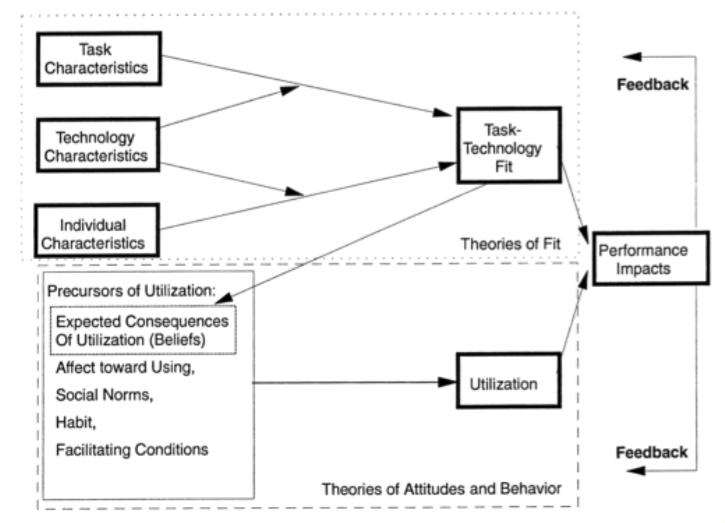
\includegraphics[width=\textwidth]{grafiken/ttf.png}
	\caption{Task-Technology Fit model\cite{MES10}}
\end{figure}

\paragraph{Task characteristics:}
\begin{itemize}
	\item Moving responsibility for test definition from developers to management staff
	\item Reduce the time for bugs allocation and fixation
\end{itemize}


\paragraph{Technology Characteristics:}
\begin{itemize}
	\item Asynchronous software
	\item Real-time software
\end{itemize}

\paragraph{Individual Characteristics:}
\begin{itemize}
	\item  No developer background
\end{itemize}

\paragraph{Task-Technology-Fit:}
\begin{itemize}
	\item Test Sheet is a representation for tests developed with the goal to combine the power and completeness of formal programming language with a representation that is easy to understand and work with even for people with little IT knowledge\cite{ts}.
	\item node.js is an asynchronous event-driven framework designed to build scalable network applications.
	\item Optimization for real-time execution is done by changing test steps execution order and position in the event loop with the respect to their reference structure
	\item Automatization of bug reporting process directly to the developer (not covered in paper probably should not be mentioned)
\end{itemize}

\paragraph{Utilization:}
\begin{itemize}
	\item Excel UX
	\item Simple conventions
\end{itemize}

\paragraph{Performance Impact:}
\begin{itemize}
	\item Better / automated quality assurance process
	\item Wider spread of tasks and responsibility distributions amongst developers and managers
	\item Increased awareness / technical understanding of product functionality for managers 
	\item Time for training and using the test sheet required from managers
	\item Change of job descriptions / new tasks and responsibilities for managers
\end{itemize}

\section{Misfits}
\paragraph{Functionality misfits:} occur, when the way processes are executed using the ES leads to reduced efficiency and effectiveness compared to pre-ES outcomes 
\begin{itemize}
	\item No support for the data validation by the regular expressions
\end{itemize}

\paragraph{Data misfits:}  occur, when data or data characteristics stored in or needed by the ES leads to data quality issues such as inaccuracy, inconsistent representation, inaccessibility, lack of timeliness or inappropriateness for users' context
\begin{itemize}
	\item none
\end{itemize}

\paragraph{Usability misfits:}  occur, when the interactions with the ES required for task execution are cumbersome or confusing, i.e. requiring extra steps that add no value or introduce difficulty in entering or extracting information 
\begin{itemize}
	\item It is necessary to manually set define JSON object to be sent to API
	\item Test generated code must be copied to the same machine as working system
\end{itemize}


\paragraph{Role misfits} occur, when the roles in the ES are inconsistent with the skills available, create imbalances in the workload leading to bottlenecks and idle time, or generate mismatches between responsibility and authority 
\begin{itemize}
	\item Requires managements to copy up-to-date generated code to the production workstation
	\item Code generation requires call of command via CLI
\end{itemize}

\paragraph{Control misfits} occur, when the controls embedded in the ES provide too much control, inhibiting productivity, or too little control, leading to the inability to assess or monitor performance appropriately 
\begin{itemize}
		\item Business staff has an access to the production environment 
		\item It is necessary to manually set define JSON object to be sent to API
\end{itemize}


\paragraph{Organizational culture misfits}  occur, when the ES requires ways of operating that countervene organizational norms 
\begin{itemize}
	\item The fact that test steps defined by non-developers staff confuses developers
\end{itemize}


\section{Benefits and affecting factors}
\paragraph{Organizational benefits} from the system use from the perspective of senior management, is an overall measure of senior managemt's perception of the benefits from the IT-based application. Such benefits - which may be assessed either for the enterprise system investment overall, or from the individual enterprise system projects - usually revolve around the software enabling the faster and more accurate process of coordination and execution, including links with business partners up and down the supply chain and the greater accuracy of and visibility into organizational data, resulting in more tightly controlled organizational processes improved asset utilization and improved decision making.

\subsection{Short-term factor}
\paragraph{Functional Fit} is the extent to which the functional capabilities embedded and congigured within an enterprise system packge match the functionality that organization needs to operate effectively and efficiently. Saying that software has good functional fit is equivalent to saying that the processes supported by system are efficient and effiective for the organization and the software helps people in organization get their jobs done. It conceptualized as being delivered and measured project by project.
\paragraph{Overcoming Organizational Inertia} is the extent to which members of the organization have been motivated to learn, use, and accept new system. During initial implementation and subsequent upgrade projects, considerable change-management effort, training, and support are needed to overcome organizational inertia.

\subsection{Long-term factor}
Can not be discovered due to the time constraints on the research project.
\paragraph{Integration} of information system is the unification of processes and/or data from multiple computer-based systems, not necessarily in the one organization.
\paragraph{Process optimization} is any attepmt to improve the efficiency and effectiveness of an organizations processes, ultimately in support of strategic goals.
\paragraph{Improved access to information} is any step taken to increase the provision of timely, accurate, relevant information to key organizational decision making.
\paragraph{On-going major enterprise system improvement projects} is a measure of the number and the extent of investment in major business improvement projects that an organization has undertaken for improving and extending its enterprise system. Major business projects are those that lead to changes in the way that work is done in the business.

\paragraph{Operational Benefits of Test Sheets Use}
\begin{itemize}
	\item Feedback cycle time reduction;
	\item Productivity improvement - Developers can concentrate more on creating and fixing code instead of running manual tests
	\item Quality improvement - Errors are identified earlier due to automated monitoring, bugs are easier identified before deployments
	\item Customer Service improvement - Less complaints from customers (!not descriptive "LESS")
\end{itemize}

\paragraph{Managerial:}
\begin{itemize}
	\item Resource management - No additional QA staff necessary
\end{itemize}

\paragraph{Organizational:}
\begin{itemize}
	\item Changing work patterns - Reduced workload on developers, increased product quality responsibility for managers
	\item Facilitating organizational learning - Managers learn / gain more technical understanding and feel empowered by owning the responsibility for the testing
\end{itemize}
%\begin{table}[h]
%	\begin{center}
%		\begin{tabular}{| l | l |  }
%			\hline
%			\textbf{Cost reduction} & +  \\
%			\hline
%			\textbf{Cycle time reduction} & + \\
%			\hline
%			\textbf{Productivity improvement} & +  \\
%			\hline
%			\textbf{Quality improvement} & + \\
%			\hline 
%			\textbf{Customer Service improvement} & + \\
%			\hline
%		\end{tabular}
%	\end{center}
%	\caption{Operational Benefits of Test Sheets Use}
%\end{table}
%
%\begin{table}[h]
%	\begin{center}
%		\begin{tabular}{| l | l |  }
%			\hline
%			\textbf{Resource management} & +  \\
%			\hline
%			\textbf{Decision making and planning} & + \\
%			\hline
%			\textbf{Performance} & +  \\
%			\hline
%		\end{tabular}
%	\end{center}
%	\caption{Managerial Benefits of Test Sheets Use}
%\end{table}
%
%\begin{table}[h]
%	\begin{center}
%		\begin{tabular}{| l | l |  }
%			\hline
%			\textbf{Business growth} & +  \\
%			\hline
%			\textbf{Business alliance} & + \\
%			\hline
%			\textbf{Building business innovations} & +  \\
%			\hline
%			\textbf{Building cost leadership} & + \\
%			\hline 
%			\textbf{Product differentiation} & + \\
%			\hline
%			\textbf{External linkages} & + \\
%			\hline
%		\end{tabular}
%	\end{center}
%	\caption{Strategic Benefits of Test Sheets Use}
%\end{table}
%
%\begin{table}[h]
%	\begin{center}
%		\begin{tabular}{| l | l |  }
%			\hline
%			\textbf{Business flexibility for future challenges} & +  \\
%			\hline
%			\textbf{IT cost reduction} & + \\
%			\hline
%			\textbf{IT infrastructure capabilities} & +  \\
%			\hline
%		\end{tabular}
%	\end{center}
%	\caption{IT infrastructure Benefits of Test Sheets Use}
%\end{table}
%
%\begin{table}[h]
%	\begin{center}
%		\begin{tabular}{| l | l |  }
%			\hline
%			\textbf{Changing work patterns} & +  \\
%			\hline
%			\textbf{Facilitating organizational learning} & + \\
%			\hline
%			\textbf{Empowerment} & +  \\
%			\hline
%			\textbf{Building common vision} & + \\
%			\hline
%		\end{tabular}
%	\end{center}
%	\caption{Organizational Benefits of Test Sheets Use}
%\end{table}


